\documentclass{rbfin}
\usepackage{amsmath}
\usepackage{amssymb} %mathbb
\usepackage{gensymb} % \degree
\usepackage{graphicx}
\usepackage{hyperref}
\usepackage{cancel}
\newcolumntype{C}{>{$}c<{$}}


\begin{document}
\selectlanguage{brazil}
\shorttitle{Identificação de Sistemas e Estimação de Parâmetros 2022} % appears on header every other page
\rbfe{}
\autor{Vinícius Claudino Ferraz, 2022}


\large

\begin{center}
LISTA 1
\end{center}

\normalsize

\doublespacing

\section*{Questão 1}

a) Abaixo o gráfico de $u$, para $T_s = 0.1$ segundo.

\begin{center}
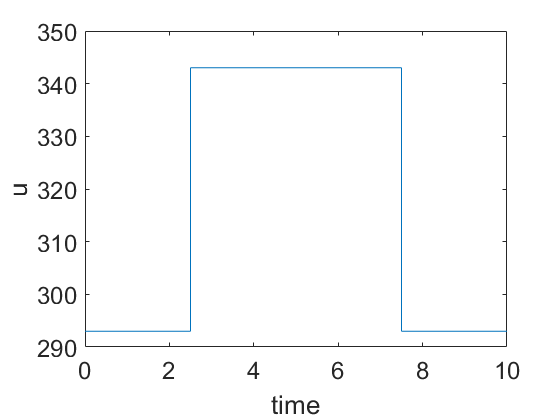
\includegraphics[scale=0.666]{q1a}
\end{center}

b) Abaixo o gráfico de $y$.

\begin{center}
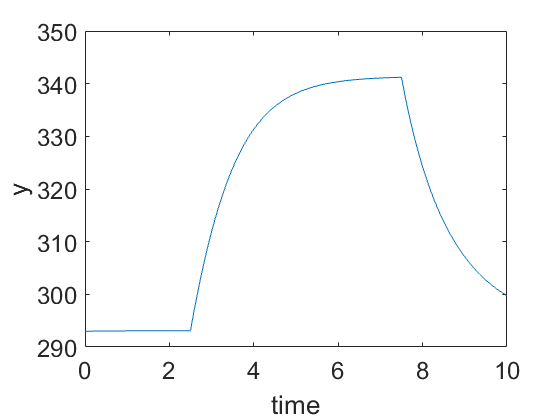
\includegraphics[scale=0.666]{q1b}
\end{center}

\newpage

\section*{Questão 2}

a) Abaixo o gráfico de $u$, para $T_s = 10$ segundos.

\begin{center}
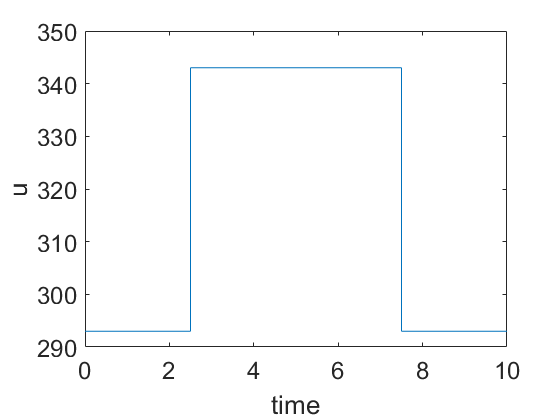
\includegraphics[scale=0.666]{q2a}
\end{center}

b) Abaixo o gráfico de $y$:

\begin{center}
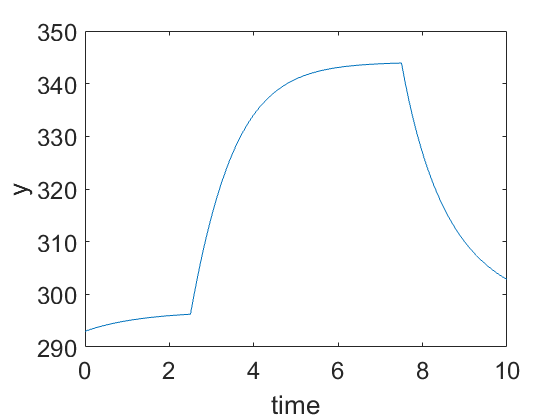
\includegraphics[scale=0.666]{q2b}
\end{center}

\newpage

c) Abaixo a comparação, considerada uma constante igual a $3000$:

\begin{center}
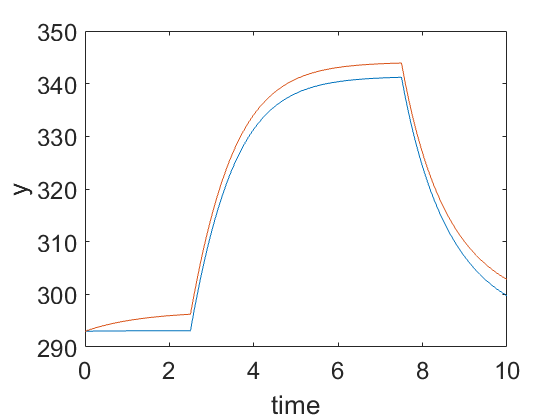
\includegraphics[scale=1]{comparacao}
\end{center}

Como vemos, a forma dos sinais é semelhante. Acreditamos que a diferença seja graças aos tempos diferentes de amostragem.

\section*{Questão 3}

a) O primeiro modelo é não linear, pelo termo $u$ multiplicado por $y'(t)$, ao contrário do segundo, em que $y'(t)$ é multiplicado por uma constante. Além disso, aplica-se facilmente a transformada de Laplace no segundo modelo e consegue-se a função de transferência $H(s) = \cfrac{K}{\tau s + 1}$.

Seja $y_1$ a solução de: $5 u(t) \cfrac{dy}{dt} + y(t) - 10 u(t) = 0 \Rightarrow \cfrac{dy}{dt} = 2 - \cfrac{y(t)}{u(t)}$.

Como vemos na figura abaixo, para degraus de altura sempre a mesma, o tempo necessário para atingir o estado estacionário aumenta: 

\begin{center}
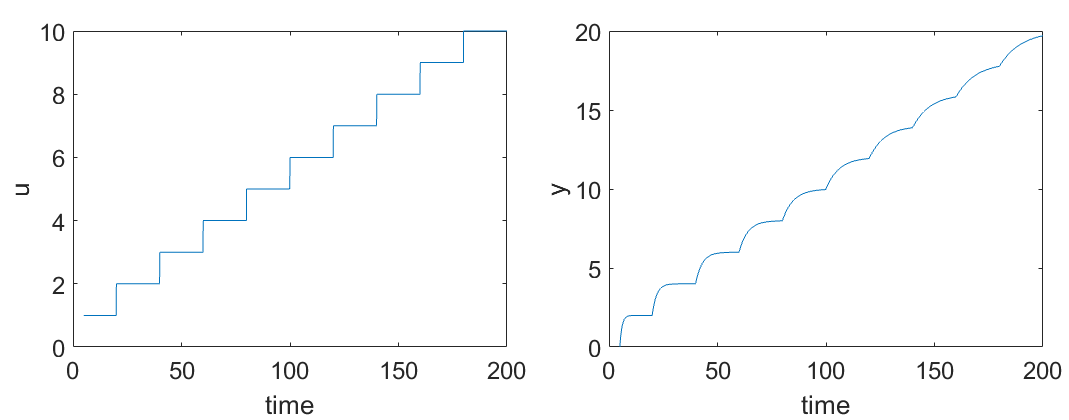
\includegraphics[scale=0.65]{q3y1}
\end{center}

Portanto o modelo é não linear.

Seja $y_2$ a solução de: $5 \cfrac{dy}{dt} + y(t) - 10 u(t) = 0 \Rightarrow \cfrac{dy}{dt} = \cfrac{10 u(t) - y(t)}{5}$.

Como vemos na figura abaixo, para degraus de altura sempre a mesma, a forma da saída é sempre a mesma, para todo ponto de operação: 

\begin{center}
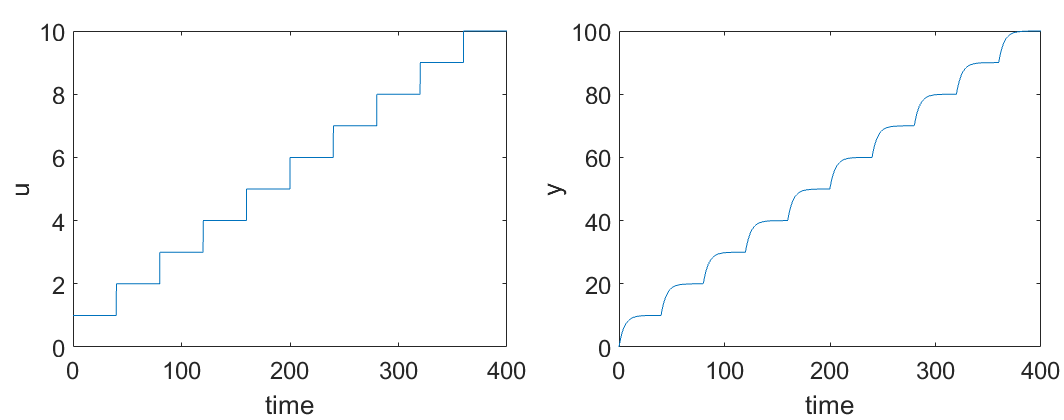
\includegraphics[scale=0.65]{q3y2}
\end{center}

Portanto o modelo é linear.

b) Pela função de transferência $H(s)$, temos que $\tau$ é a constante de tempo de $y_2$. À medida que $\tau \to 0$, o módulo do expoente aumenta. À medida que $\tau \to \infty$, o expoente tende a $1$ e a resposta ao impulso tende a ficar constante.

No primeiro sistema, $\tau(u) = 5 u(t)$, aproximadamente. A constante de tempo depende do próprio $u$, como uma velocidade com que o sistema responde a variações na entrada. Quanto mais $\tau(u)$ próximo de uma constante, mais próximo de linear o sistema.

c) $H(s) = \cfrac{K/\tau}{s + 1/\tau}$. Pela transformada de Laplace inversa, $h(t) = \cfrac{K}{\tau} \exp(-t/\tau), t \ge 0$.

Creio não ser possível calcular facilmente a transformada de Laplace do produto $u(t) y'(t)$.

\vspace{6mm}

Versão de 22/abril/2022\footnote{Fora da caridade não há salvação.} por Vinicius Claudino Ferraz. 

Matrícula: 2019435823.

\end{document}
